\documentclass[12pt, block=fill]{beamer} 
\usepackage[sfdefault]{FiraSans}
\usepackage{FiraMono}
\usepackage[T1]{fontenc}
\usepackage{xcolor}

\usepackage{pgfpages}
\setbeameroption{hide notes} % Only slides
% \setbeameroption{show only notes} % Only notes
  % \setbeameroption{show notes on second screen=right} % Both

\definecolor{burntOrange}{rgb}{.8, .5, .1}
\definecolor{textgray}{rgb}{.8,.8,.8}

\usetheme[titleformat frame = smallcaps]{metropolis}

\metroset{block=fill}

\newcommand{\E}{\text{E}}
\newcommand{\V}{\text{V}}
\newcommand{\cov}{\text{cov}}

% \title{Week 6}
% \subtitle{Hypothesis Testing}

% \author{Paul Laskowski and D. Alex Hughes}
% \institute{UC Berkeley, School of Information}

\begin{document}

% \begin{frame}
% \maketitle
% \end{frame}

\section{A Tale of Two Statistics}

\begin{frame}
  A hypothesis, \textbf{H}, is a model for how the world might work.

  In practice, evidence is rarely conclusive.

  \begin{itemize}
    \item We would like to know, $P(H|D)$. That is, the probability that our hypothesis is true, given the data that we observe from the world.
    \item But there is a fundamental dilemma: We will never know whether our hypothesis is true.
    \item The world isn't a perfect laboratory, and although we can collect evidence and information, this evidence cannot identify a single, \textit{unique} model from the set of all possible models.
    \item We cannot make a probability statement about the models either!
  \end{itemize}
\end{frame}

\begin{frame}
  \frametitle{Example 1: Coin Flips}
  Suppose that you flip a coin once and it lands heads. \textit{What is the probability that it is a double-headed coin?}

  \begin{itemize}
    \item Is there enough information to answer this question?
    \item How did the coin get there? The context is missing?
    \item Even with more information, we still cannot ever possess the \textit{entire} context.
  \end{itemize}
\end{frame}

\begin{frame}
  \frametitle{Example 2: Gravity}
  \begin{itemize}
    \item Both motions are constant with a gravitation attraction that is proportional to the square of the distance between two objects.
    \item What is the probability that Newton's theory of gravity is ``correct''?
  \end{itemize}

  \textbf{Problem:} Newton's theory seemed to work well up to the precision of 17th-century instruments.

  \begin{itemize}
    \item But, it is the present now, and we have developed instruments that pretty clearly say that Newton's laws are incorrect.
    \item How could Newton decide how likely was his model compared to general relativity (which hadn't even been imagined yet!)?
  \end{itemize}
\end{frame}

\begin{frame}
  \frametitle{Example 2: Take-away}
  We can never write down the infinite number of models that are possible consistent with our observations. And, even if we could, we could not assign a probability distribution to these models.
\end{frame}

\begin{frame}
  \frametitle{Example 3: Giant Squid }
  Suppose that you discover three new specimens of a new squid species that measure 3.2, 3.3, and 4.0 feet long.

  \begin{itemize}
    \item What is the probability that the average length among the entire species is 3.5 feet?
    \item Probability is zero for a single point (continuous probability measures).
    \item Probability that the average length is between 3 and 4 feet?
  \end{itemize}

  What we know and don't know:
  \begin{itemize}
    \item We know about our \textit{sample}.
    \item We do not know about our \textit{population}.
  \end{itemize}
\end{frame}

\begin{frame}
  \frametitle{Two Branches of Statistics }
  \centering
  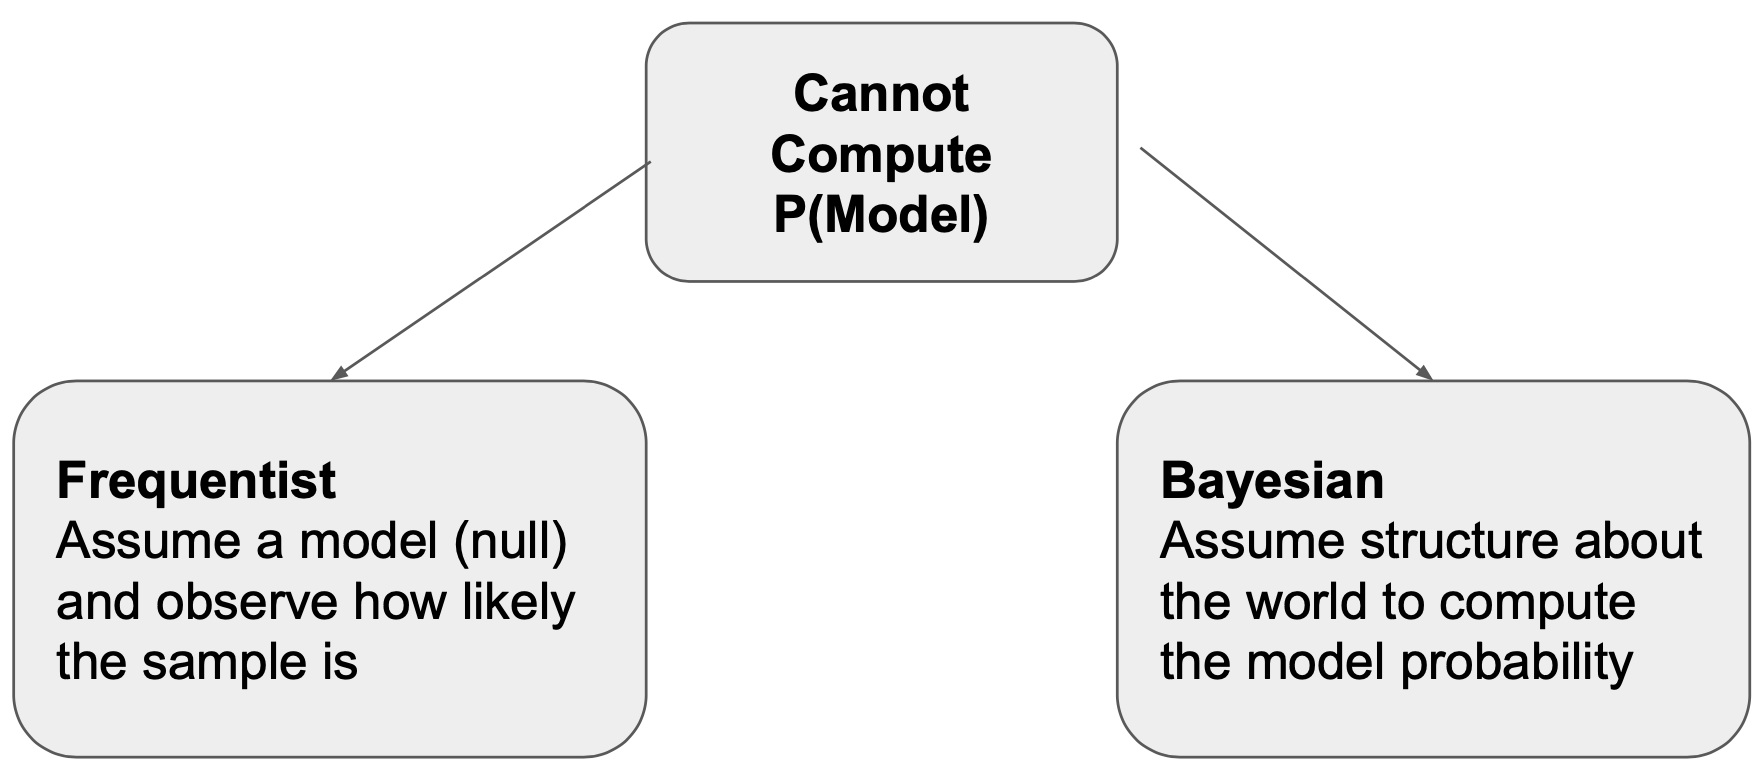
\includegraphics[width=.9\linewidth]{./figures/two_worlds}
\end{frame}

\section{The Frequentist Approach}

\begin{frame}
  \frametitle{The Birth of Modern Statistics}
  \textbf{Before the 1930s}
  \begin{itemize}
    \item Many ``statistical'' procedures; but, no coherent account of how to choose one.
    \item Neyman and Pearson published articles that added a formal mathematical treatment, laying the foundations for frequentist statistics.
  \end{itemize}
\end{frame}

\begin{frame}
  \frametitle{The Central Dilemma}

  Despite the ``modern'' development of statistics, there is a problem.

  \begin{itemize}
    \item We observe data, $D$.
    \item Given the data that we observe, we \textit{would like to know} the probability that our hypothesis is true.
    \item That is, $P(H|D)$.
  \end{itemize}

  But, frequentist statistics:

  \begin{itemize}
    \item Not only cannot compute this probability.
    \item Doesn't think it even makes sense to assign a probability to a hypothesis.
  \end{itemize}
\end{frame}

\begin{frame}
  \frametitle{Objective Probability}

  A frequentist defines probability as a matter of long-run frequencies.

  \begin{itemize}
    \item Frequentists specify a collective of elements (e.g. experiments, or throws of dice).
    \item As the number of observations approaches infinity, the proportion of the throws that show a $3$ is $\frac{1}{6}$.
    \item For frequentists, \textbf{objective probability} is this long-run frequency of the event.
  \end{itemize}
\end{frame}

\begin{frame}
  \frametitle{Objective Probability and Hypotheses}
  \begin{itemize}
    \item If one views probability as objective, then they cannot talk about the probability of a hypothesis.
    \item A hypothesis is just a statement that is either \textit{TRUE}, or \textit{FALSE}.
    \item This mixes language a little, but when one talks about the probability of a hypothesis, they are talking about \textbf{subjective probability}, which is not the purview of data science.
  \end{itemize}
\end{frame}

\begin{frame}
  \frametitle{What Probabilities Can We Study?}
  We can study events that have (or could have) a long-run collective.

  $$
  P(D|H)
  $$

  where $H$ is a hypothesis and $D$ is data.

  \begin{itemize}
    \item Assume that $H$ is true, and call it the null hypothesis.
    \item Has to be \textit{very} specific.
    \item Is the basis for predictions we need to make about the data that ``should'' come out of the experiment (if this $H$ were actually true).
  \end{itemize}
\end{frame}

\begin{frame}
  \frametitle{An Imprecise Statement}
  Vitamin W kicks the bad toxins right smack outta your system. (Read this like a TV salesperson.)
\end{frame}

\begin{frame}
  \frametitle{A Precise Statement }
  Vitamin W reduces blood pressure by 12 mmHg on average.

  \begin{itemize}
    \item With a precise statement, we also have a statement about the data that \textit{should} be observed; and so,
    \item We have a collective to produce a long-run frequency, i.e. a probability.
  \end{itemize}
\end{frame}

\section{Decision Rules}

\begin{frame}
  \frametitle{Hypothesis Test Example}

  \begin{exampleblock}{Mad data science}
    Suppose that your lab has synthesized a new compound, 
    \textit{Vitamin W}.

    Let random variable $B$ represent the change in blood pressure that results from taking
    \textit{Vitamin W}.
    
    Let $\mu = \E[B]$.

    You need to make a decision, to invest resources in Vitamin W or not. 
  \end{exampleblock}
  
  \note[item]{Let's use a stylized example to motivate the hypothesis testing framework.}
   
 \end{frame}

\begin{frame}
  \frametitle{Two Possible States of the World}
  \textbf{Goal:} Begin with a reasonable default supposition; leave
  this supposition behind if data provides compelling evidence
  \begin{columns}[t]
    \column{.5\linewidth}
    \textbf{Null hypothesis}
    \begin{itemize}
    \item Default assumption, status quo, statement that data might overturn
    \item  $H_\varnothing: \text{Usually } \mu=0$
    \item No effect
    \end{itemize}
    \column{.5\linewidth}
    \textbf{Alternative hypothesis}
    \begin{itemize}
    \item Idea or alternative to status quo
    \item $H_a:$ Usually  $\mu \neq 0$
    \item Some effect exists
    \end{itemize}
  \end{columns}
  
  With compelling evidence, we leave the specific null hypothesis
  ($H_{\varnothing}$) for the alternative ($H_{a}$)
\end{frame}

\begin{frame}
\frametitle{A Hypothesis Test}

A \textit{hypothesis test} is a procedure.

\begin{center}
  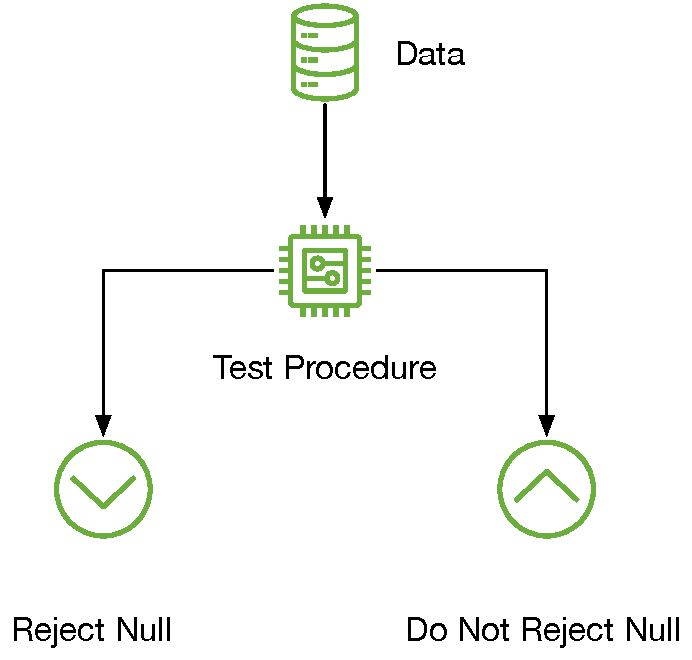
\includegraphics[width=.65\textwidth]{figures/test_procedure}
\end{center}
\note[item]{This is very strict: you might want your hypothesis test
  to do more, to give you fine-grained information about the world.
  but statistics doesn't work like that.  All we can do, is set up a
  specific null hypothesis and make this binary decision: reject or
  not reject.} 
\end{frame}


\begin{frame}
  \frametitle{False Positive and False Negative Errors}
  \begin{center}
    \small
    \begin{tabular}{p{3cm}| p{3cm}| p{3cm}}
      & \multicolumn{2}{c}{\textbf{True state of the world}}  \\ 
      & \textit{The null is true} & \textit{The null is false} \\
      \hline \hline 
      \textit{Reject the null} & False Positive & \\
      & (Type I Error) & \\
      \hline 
      \textit{Do not reject the } & & False Negative\\
      \textit{null}&& (Type II Error)
    \end{tabular}
  \end{center}
\end{frame}

\begin{frame}
  \frametitle{False Positive and False Negative Errors (cont.)} 
  \textbf{False Positive Errors}
  \begin{itemize}
    \item Typically the most destructive
    \note[item]{Why?  Because we don't want to abandon our existing
      beliefs about the world too quickly - our existing beliefs are
      our beliefs for a reason.}
    \note[item]{The world has all these researchers testing different
      medications, we don't want to be flooded with treatments that
      don't actually work.}
    \note[item]{Once a single study finds a link between red wine and
      heart disease, it gets out into the papers, people start
      believing it, and there's no way to undo that. }
  \item Error rate, denoted $\alpha$, is the probability of rejecting
    the null hypothesis when we should not; $P(\text{Reject } H_\varnothing |
    H_\varnothing)$
  \item Starting with Ronald Fisher: set $\alpha = 0.05$
  \end{itemize} 
  
  A hypothesis test is a procedure for rejecting or not rejecting a
  null, such that the false positive error rate is controlled ($\alpha = 0.05$).
\end{frame}


\begin{frame}
  \frametitle{Breaking Down a Test Procedure}
  
  \textbf{A test statistic}
  \begin{itemize}
  \item A function of our sample
  \item Measures deviations from the null hypothesis
  \item Distribution must be completely determined by the null
  \end{itemize}

  \textbf{A rejection region}
  \begin{itemize}
  \item  A set of values for which we will reject the null
  \item  Chosen to be contrary to the null
  \item Total probability must be $\alpha = 0.05$
  \end{itemize}
\end{frame}

\begin{frame}
  \frametitle{What a Hypothesis Test Doesn't Do}

  \textbf{A hypothesis test does not prove the null hypothesis.}
  
  \begin{itemize}
  \item We control Type 1 error rates
    \note[item]{Throughout, can we refer to these as false positives
      and false negatives? Or, at the very least, can we be really
      clear about defining once what we mean by type-one and type-two
      errors? This is a pet peeve of mine.} 
  \item We cannot control Type 2 error rates
  \item How can you be sure the real B is not 0.01?  Or 0.00001?
    \note[item]{I'm not sure what we mean with this last point?} 
  \end{itemize}
  
    \textbf{Never accept the null hypothesis.}
\begin{itemize}
\item The valid decisions are reject and fail to reject.
\end{itemize}

  
\end{frame}

\section{The One-Sample z-Test}

\begin{frame}[t]
  \begin{exampleblock}{Vitamin W Example} 
    Suppose $(B_1,..,B_{100})$ are i.i.d. random variables with mean $\mu = \E[B]$, representing changes in blood pressure.
    
    Assume $B \sim N(\mu, \sigma)$.  Assume we know $\sigma[B]=20$.
      \end{exampleblock}
      
      \note[item]{We want to know if Vitamin W has an effect.  so we write $H_0: \mu = 0$.}
      \note[item]{We need a statistic, and a rejection region}
      \note[item]{For our statistic, we usually want to find something that follows a famous distribution.}
      \note[item]{Can use the standardized mean. $z = \frac{\bar{B}}{2} \sim N(0,1)$}
\note[item]{For our rejection region , we need to choose a subset of the real numbers.  I'll show you the most common choice, above 1.96 and below -1.96.}
\note[item]{Why these numbers?  If you integrate, you get a probability of 0.05.}
\note[item]{Ex: $\overline{B} = -5$. then $z = 2.5$ REJECT}
\vspace{.5cm}
   \begin{flushright} 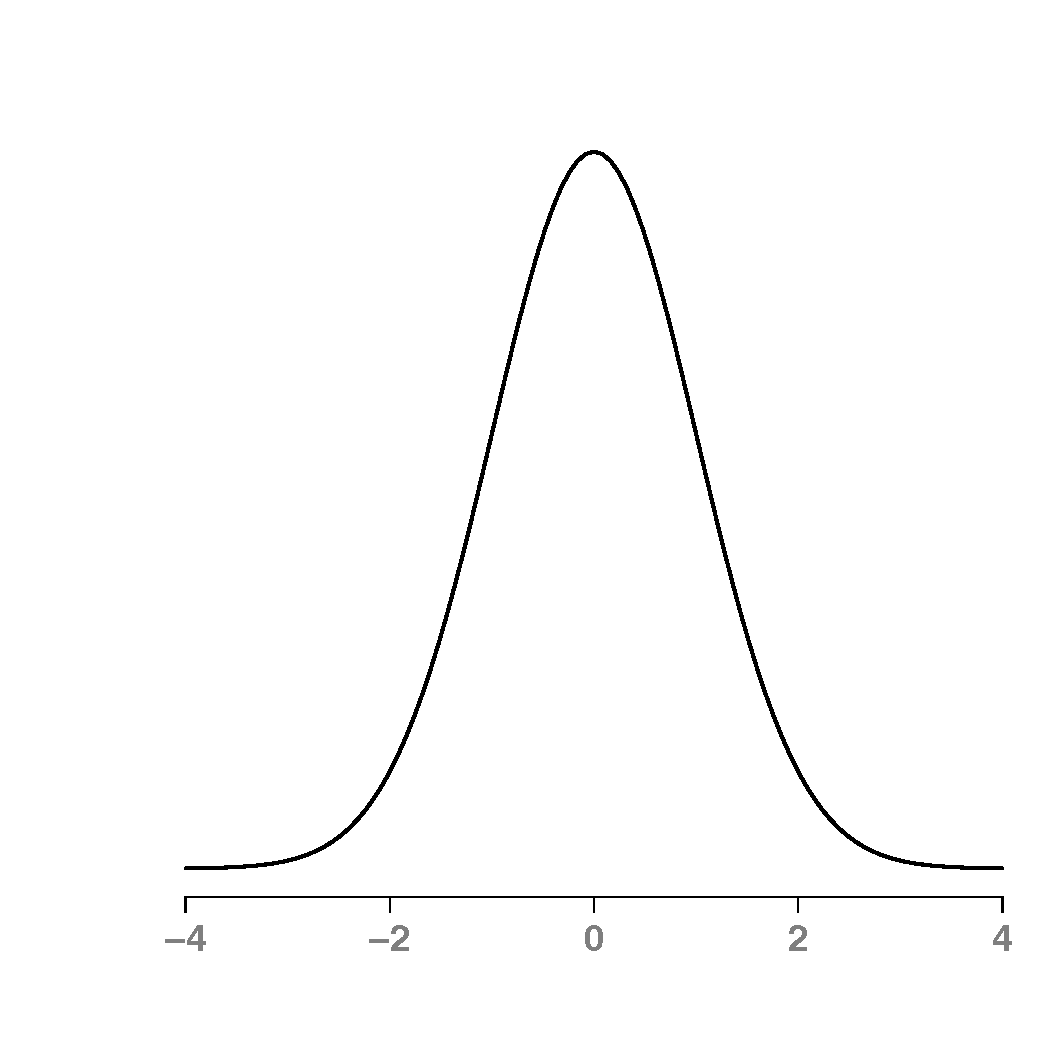
\includegraphics[height=.5\textheight, width = .5\textwidth]{figures/normal.pdf}
\end{flushright}
\end{frame}




% \section{Decision Rules Concept Check}

% \begin{frame}
%   \frametitle{Decision Rules Concept Check}

%   \begin{exampleblock}{A magician}
    
%     A magician gives you a coin. You want to run a test to see if it
%     is a fair coin.
% 
%     Your null hypothesis is that the coin is fair, and so has a
%     probability of heads that is $1/2$.
% 
%     You decide that you are going to flip the coin five times and declare
%     the coin to be unfair if the total number of heads is either zero
%     or five. \textbf{What is the Type 1 (false positive) error rate
%     for your procedure?}
% 
%     \begin{itemize}
%     \item $2 / 32$ 
%     \item $1 / 10$
%     \item $1 / 2$
%     \item $30 / 32$
%     \end{itemize}
%    
%   \end{exampleblock}
% \end{frame}

% \begin{frame}
%   \frametitle{Decision Rules Concept Check (cont.)}

%   \begin{exampleblock}{A magician}
%     \begin{itemize}
%     \item $\mathbf{2 / 32}$ -- There are 32 ways that the coins
%       \textit{might} fall, each of them equally probable. If the coin
%       \textit{were} fair in this is your rejection criteria, then you
%       will be wrong 2 of the 32 times.
%       \item $1 / 10$
%       \item $1 / 2$
%       \item $30 / 32$
%         
%       \end{itemize} 
%     \end{exampleblock}
% 
% \end{frame} 

\section{One- and Two-Tailed Tests}

\begin{frame}
  \frametitle{The Two-Tailed z-Test}

\begin{center} 
    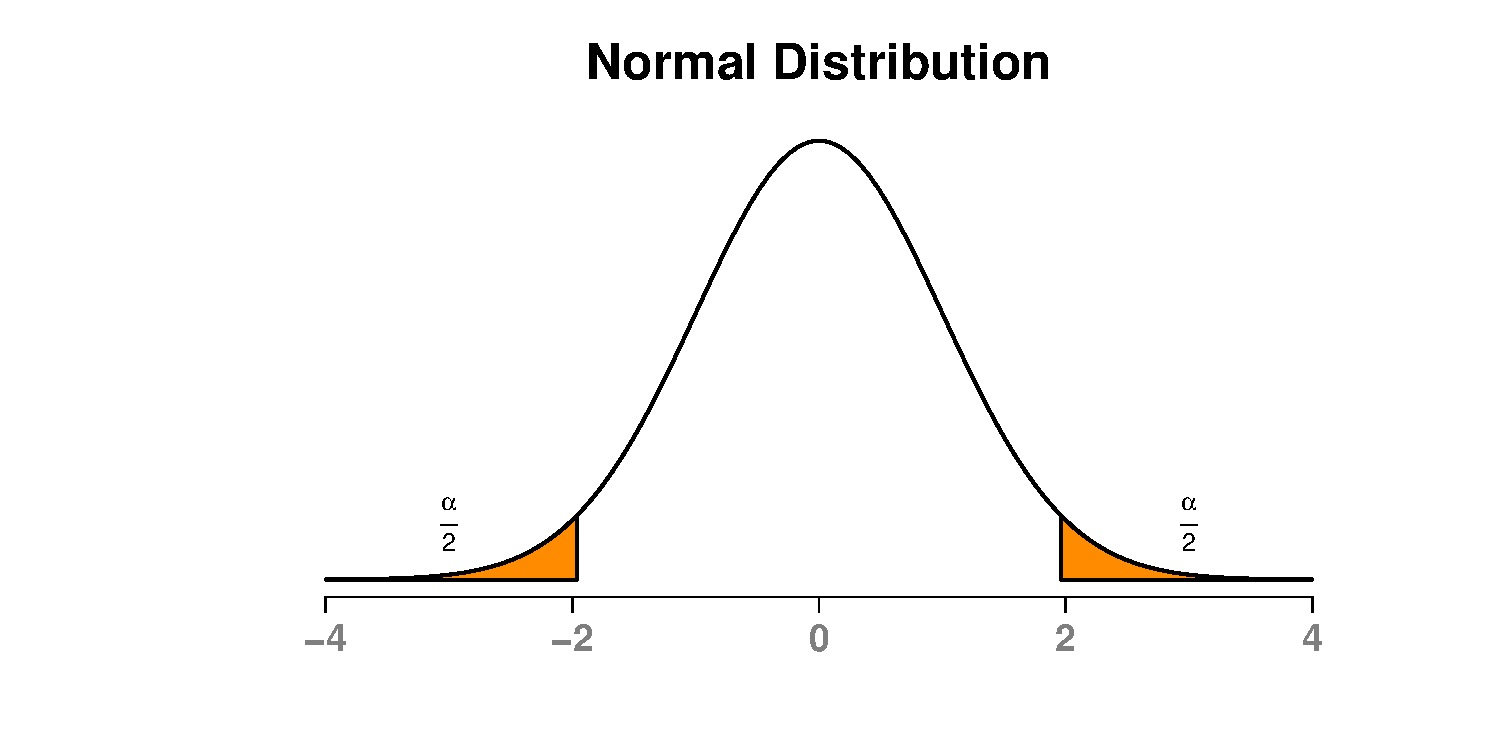
\includegraphics[width=\linewidth]{figures/normal_with_two_tails}
  \end{center}
  \begin{itemize}
  \item \textbf{Null hypothesis}: $\mu = 0$
  \item \textbf{Alternative hypothesis}: $\mu \neq 0$
  \end{itemize} 
\end{frame}

\begin{frame}
  \frametitle{The One-Tailed z-Test}
  \begin{center}
    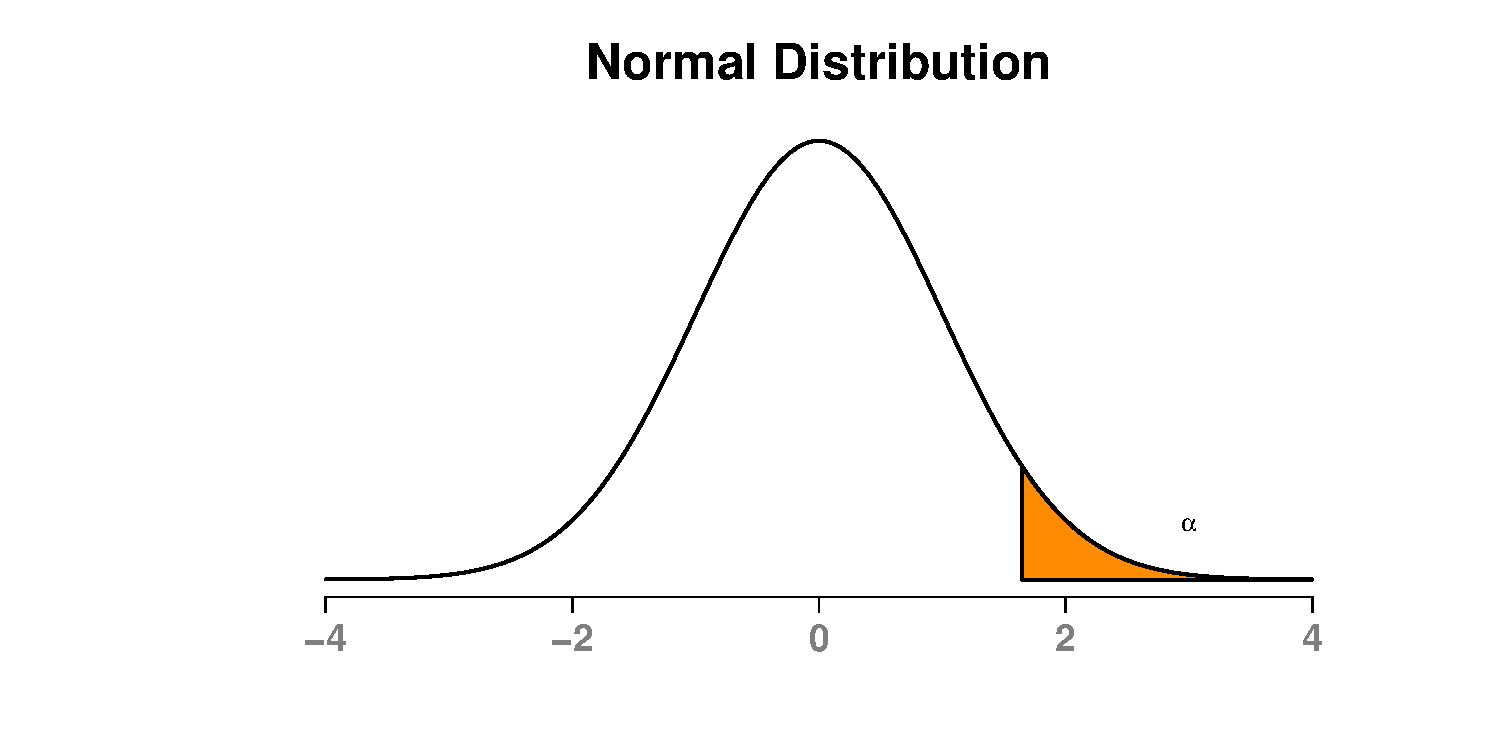
\includegraphics[width=\linewidth]{figures/normal_with_one_tail}
  \end{center}
  \begin{itemize}
  \item \textbf{Null hypothesis}: $\mu = 0$
  \item \textbf{Alternative hypothesis 1}: $\mu > 0$
  \item \textbf{Alternative hypothesis 2}: $\mu < 0$ 
  \end{itemize}
\end{frame}

\begin{frame}
  \frametitle{Choosing One or Two Tails} 

  \note[item]{One-tailed and two-tailed tests ask different questions, and are
  \textit{not} interchangeable.}
  \note[item]{It is kind of like being ID when you're buy a beer --
    they're not asking, ``Is this person different from 21?'' They're
    asking, ``Is this person older than 21?''}

  \begin{center}
    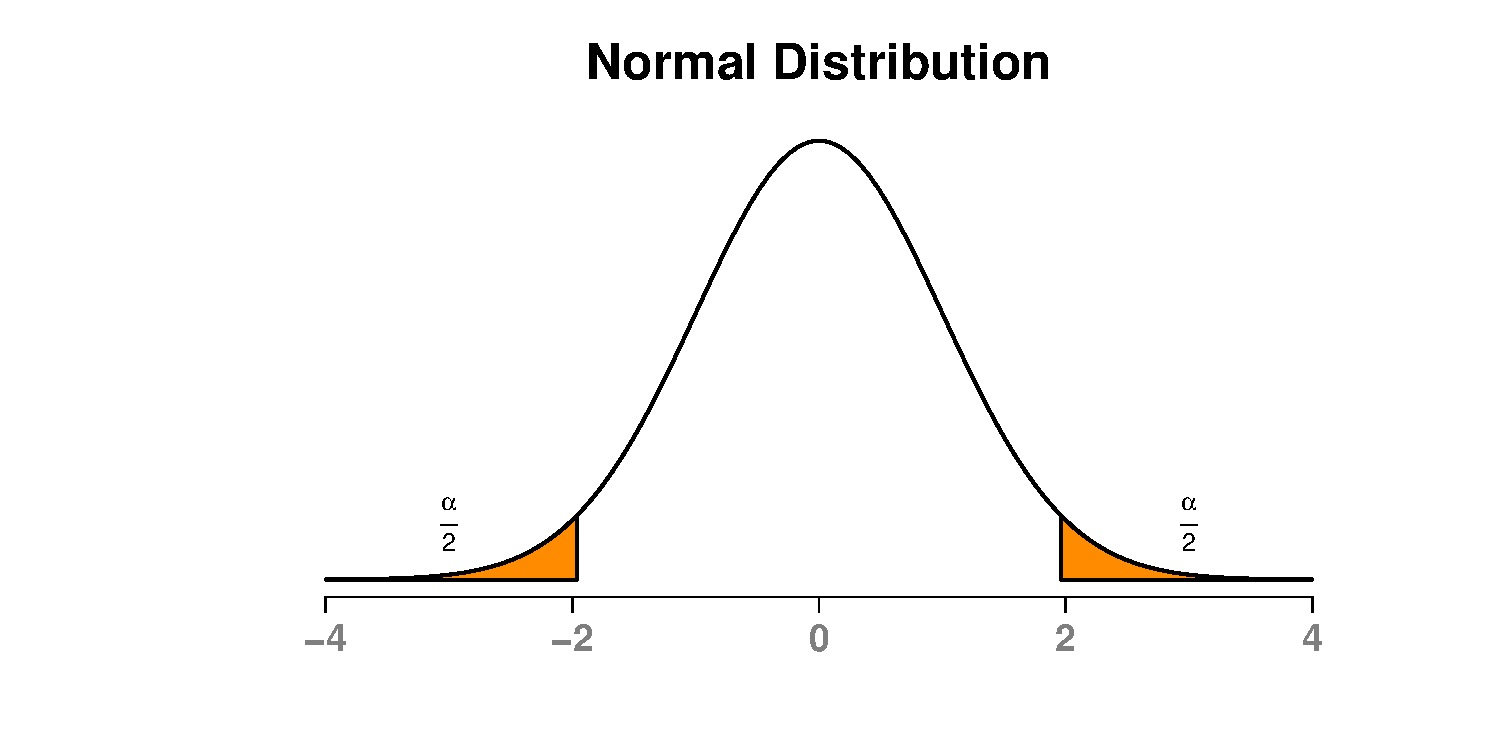
\includegraphics[width=0.6\textwidth]{figures/normal_with_two_tails} \\
    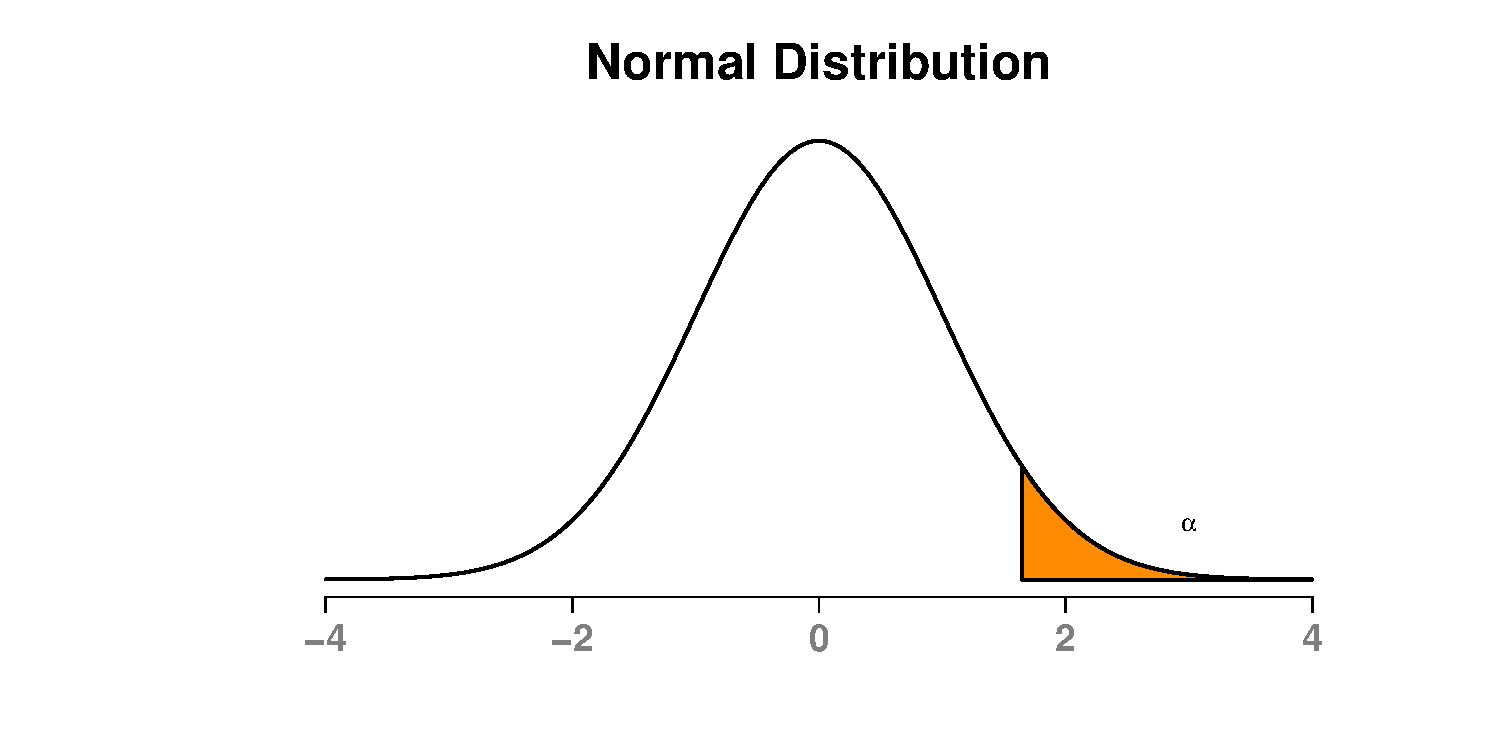
\includegraphics[width=0.6\textwidth]{figures/normal_with_one_tail}
  \end{center}

Switching your test after you see the statistic is cheating.
\end{frame}


\begin{frame}
\frametitle{One-Tailed Test: Things to Consider}

Before using a one-tailed test, ask yourself these questions:
\note[item]{``Do you feel lucky, punk? Well do ya?''}

\begin{enumerate}
\item Will the audience believe that I started with one tail before I saw the data?
\item Will the audience share my opinion of which tail is interesting?
\item Am I really 100\% committed to only this tail?
  \begin{itemize}
  \item What if the effect turns out to be huge, but in the other direction?  
  \item Would I be willing to call that a negative result?
  \item Can I convince my audience I have this much commitment?
  \end{itemize}
\end{enumerate}
\end{frame}

\section{T-Test Assumptions}

\begin{frame}
  \frametitle{T-Test Assumptions, Part I}

  \begin{block}{Assumptions of t-test}
    The textbook assumptions
    
    \begin{itemize}
    \item $X$ is a metric variable.
    \item $\{X_1,X_2,...,X_n\}$ is a random sample.
    \item $X$ has a normal distribution.
    \end{itemize}
    \end{block} 
    
    Variables are almost never normal.
    \note[item]{And so, these assumptions are nearly never met in practice}
\end{frame}

\begin{frame}
  \frametitle{T-Test Assumptions, Part II}
  
  But, in the large sample case, this is more plausible.

  \begin{block}{Large sample t-test assumptions} 
    \textbf{If}: 
    \begin{itemize}
    \item $X$ is a metric variable
    \item $\{X_1,X_2,...,X_n\}$ is a random sample
    \item $n$ is large enough that the CLT implies a normal distribution of mean
    \end{itemize}
    \textbf{Then}: The t-test is asymptotically valid
    \end{block} 
\end{frame}

\begin{frame}
  \frametitle{T-Test Assumptions, Part III}
  
\end{frame} 

\begin{frame}
  \frametitle{T-Test Assumptions, Part IV}
  
  The t-test is considered "reasonably robust," even when $n<30$, as
  long as deviations from normality are moderate.

  However, watch out for strong skewness, especially when $n<30$.

  \note[item]{DAH: We've got to give students more to work with than
    this; I think that this might end up being unsatisfying for many
    folks.} 
\end{frame}

\foreach \n in {1,...,36} {
  \begin{frame}{Gamma With Increasing Skew}
    Twenty draws from gamma distributions
    \begin{center}
      \includegraphics[width=\linewidth]{figures/gamma_skew_plots/gamma_skew_\n.pdf}
    \end{center}
  \end{frame}
}

\begin{frame}
  \frametitle{T-Test Assumptions}

  More practical guidance:
  
  \begin{itemize}
  \item $X$ is a metric variable.
  \item $\{X_1,X_2,...,X_n\}$ is a random sample.
  \item The distribution is not too non-normal, considering $n$.
  \end{itemize}
  
  When the t-test is not valid, consider using a non-parametric test instead.
\end{frame}

\section{Introduction to P-Values}

\begin{frame}
  \frametitle{Introducing P-Values}

  \begin{quote} The p-value is the probability, calculated assuming
    that the null hypothesis is true, of obtaining a value of the test
    statistic at least as contradictory to $H_0$ as the value
    calculated from the available sample.
  \end{quote}

\begin{flushright}
  \textit{ Jay L. Devore (2015)}
\end{flushright}

\note[item]{Let's note 2 things right away: just like in hypothesis
  testing.}  \note[item]{We're going to assume the null is true.}
\note[item]{We're measuring the probability of data - We may be
  interested in the probability that the null is correct - but
  statistics doesn't let us calculate that.}
\end{frame}

\begin{frame}
  \frametitle{Z-Distribution}
  
\end{frame}
  
\begin{frame}
  \frametitle{The P-Value for a Z-Test}
   
  \begin{exampleblock}{Vitamin W}
     
    You measure the effects of Vitamin W on blood pressure (measured
    in $mmHg$) for 100 patients and get $\bar{X} =3$.
     
    Assume $X \sim N(\mu,20)$.
     
    \begin{itemize}
    \item $H_0: \mu=0$
    \item $z = \frac{\bar{X} - \mu_0}{\sigma / \sqrt{n}} $
    \end{itemize}
  \end{exampleblock}
  \note[item]{ $= 3 - 0 / ( 20 / \sqrt{100} ) = 1.5$} \note[item]{$p =
    2*( 1- pnorm(1.5)) = 0.13$}
\end{frame}
 
\begin{frame}
  \frametitle{The P-Value and Decision Rules, Part I}

  Neyman-Pearson hypothesis testing: rules to make a decision and
  usually be right ($\alpha = 0.05$)

  \begin{exampleblock}{A classic z-test}
    \begin{itemize}
    \item z=1 $\rightarrow$ Do not reject null.
    \item z=2 $\rightarrow$ Reject null.
    \item z=10 $\rightarrow$ Reject null.
    \end{itemize}
  \end{exampleblock}

  \begin{itemize}
  \item Strict frequentist with a dichotomous decision rule: treat
    $z=2$ and $z=10$ identically.
  \item But is there value in knowing \textit{how contrary} the data
    is to the null?
  \end{itemize}
\end{frame}


\begin{frame}
  \frametitle{The P-Value and Decision Rules, Part II}
  \begin{align*}
    |z| & > \text{critical value} \Rightarrow \text{reject } H_{0} \\
    |z| & < \text{critical value} \Rightarrow \text{fail to reject } H_{0}
  \end{align*}

  \begin{center}
    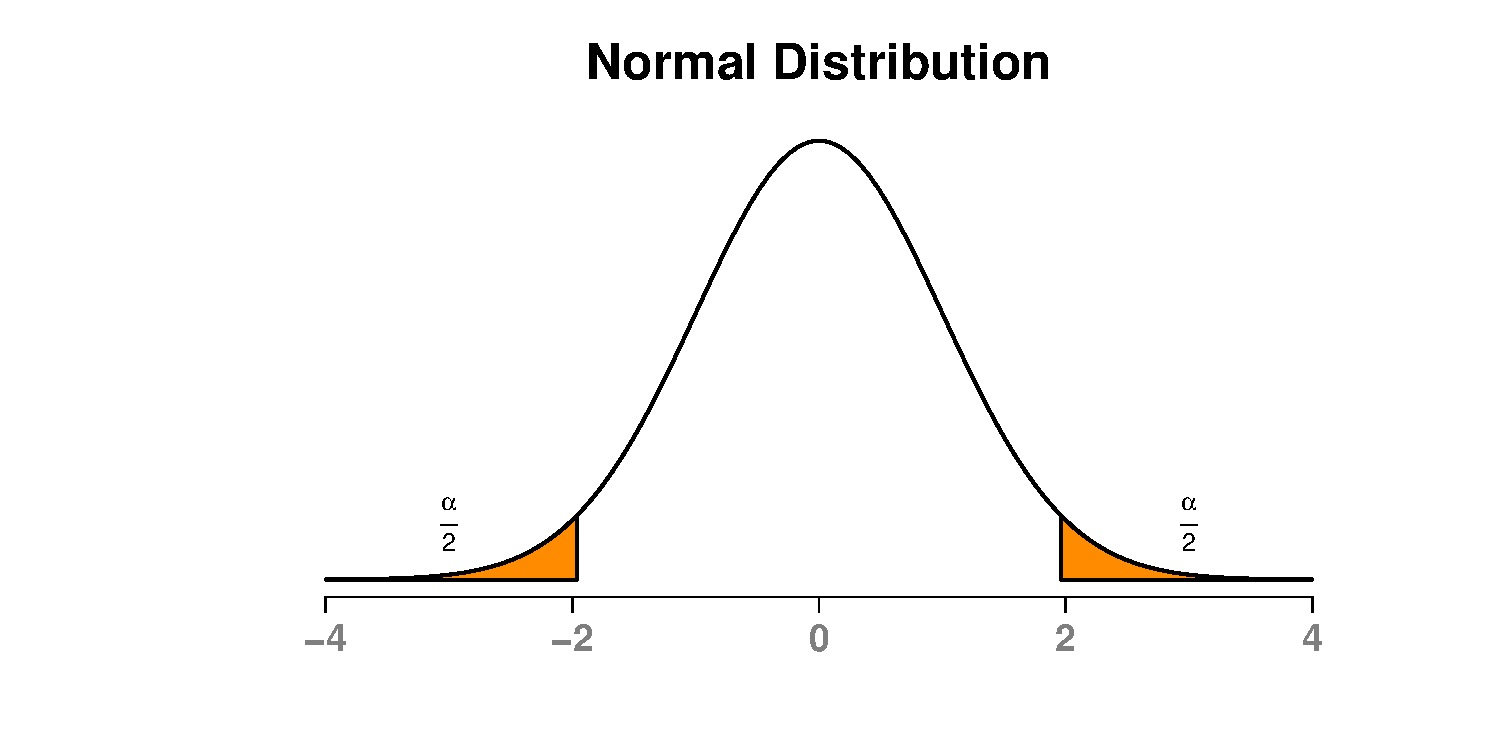
\includegraphics[width=\textwidth]{figures/normal_with_two_tails}
  \end{center}
\end{frame}

\begin{frame}
  \frametitle{The P-Value and Decision Rules, Part III}
  \begin{align*}
    |z| & > \text{critical value} \Rightarrow \text{reject } H_{0} \\
    |z| & < \text{critical value} \Rightarrow \text{fail to reject } H_{0}
  \end{align*}

  \begin{center}
    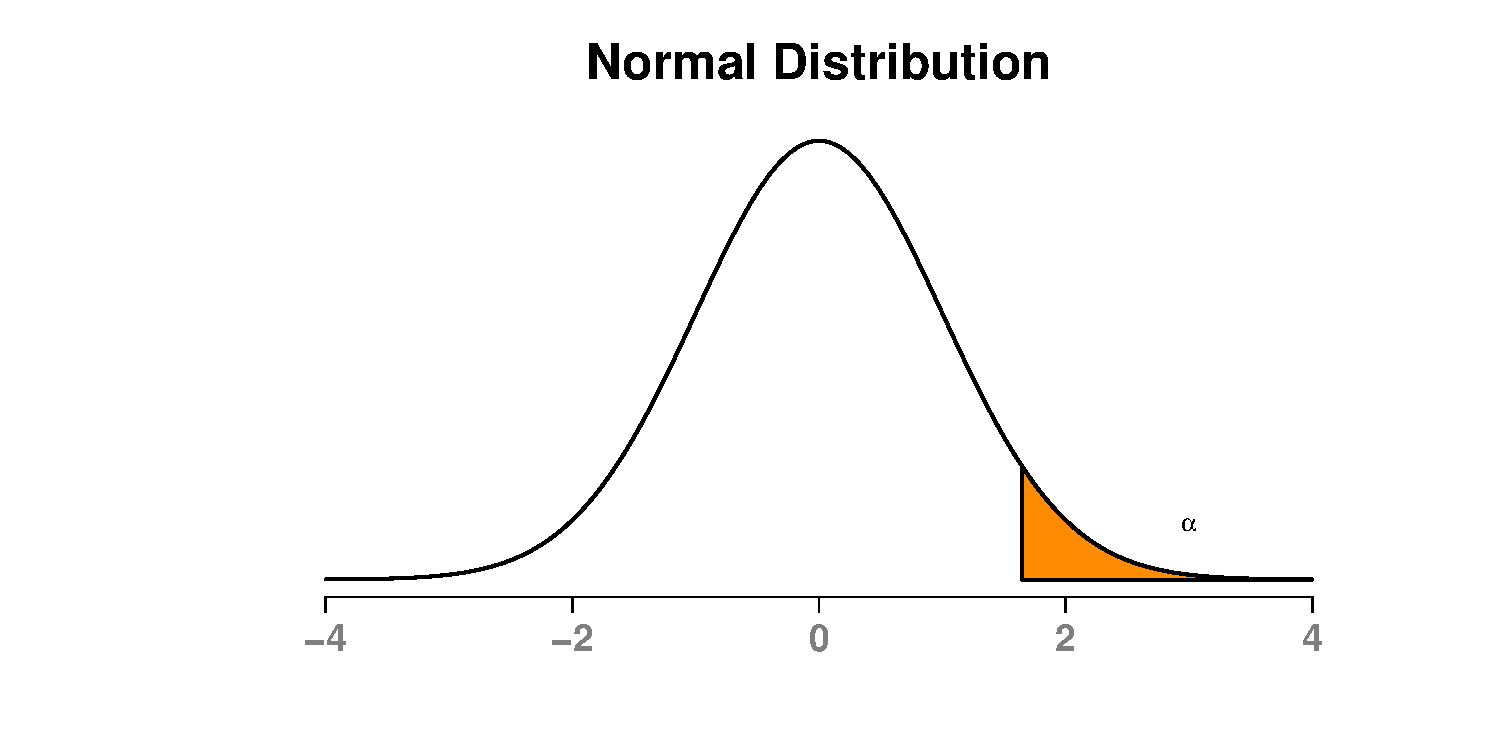
\includegraphics[width=\textwidth]{figures/normal_with_one_tail}
  \end{center}
\end{frame}

\begin{frame}
  \frametitle{An Equivalent Decision Procedure}
  
  Compute p-value.
  \begin{itemize}
  \item If $p<.05 \Rightarrow \text{reject } H_0$
  \item If $p\geq.05 \Rightarrow \text{do not reject } H_0$
  \end{itemize}
  But, can you justify making such a bright-line statement after
  reducing information so much?
  \begin{enumerate}
  \item Concept
  \item Measurement
  \item Statistic
  \item Assumptions about distribution
  \item \textbf{p-value}
  \item Reject/fail to reject
  \end{enumerate}
\end{frame}

\section{t-Test and p-Values} 

\begin{frame}
  \frametitle{P-Value Convention}
  
  \begin{center}
    \begin{tabular}{ c | c | c }
      p-value range & Convention  & Symbol \\
      \hline
      $p>0.10$ & Non-significant & \\
      \textcolor{textgray}{  $0.10 > p > 0.05$}  & \textcolor{textgray}{ Marginally-significant  } & . \\
      \hline
      $p<0.05$ & Significant & * \\
      $p<0.01$ & Highly significant & ** \\ 
      $p<0.001$ & Very highly significant & *** \\
    \end{tabular}
  \end{center}
\end{frame}
  
\begin{frame}
  \frametitle{Reporting Test Results}
  \begin{itemize}
  \item A t-test for the effect of Vitamin W on blood pressure was
    highly significant ($t=3.1$, $p=.008$).
  \item We found evidence that Vitamin W decreases blood pressure
    ($t=2.3$, $p=.04$).
  \item The effect of Vitamin X on blood pressure was not
    statistically significant ($t=1.2$, $p=.23$).
  \end{itemize}
  \vspace{.5cm}
  \begin{center}
    \begin{tabular}{ c | c }
      Vitamin W & Vitamin X \\
      \hline
      2.2 ** & 1.2 \\
      (0.6) & (0.8) \\
    \end{tabular} \\
  \end{center}

  This is half the story; next, you'll need to describe practical
  significance.

\end{frame}

\begin{frame}[t]
  \frametitle{Variable Importance and P-Values}
  Does a small p-value mean that a variable is ``important''?
  \begin{itemize}
  \item Statistical significance
  \item Practical significance
  \end{itemize} 
\end{frame} 

\begin{frame}
  \frametitle{A Warning}
  
  A very common mistake is to assume a p-value is the chance the null
  hypothesis is true.
  
  Frequentist statistics cannot tell you the probability of a
  hypothesis!

\end{frame}

\begin{frame}
  \frametitle{A Warning (cont.)}
  \begin{exampleblock}{Example}
    I test whether Vitamin X decreases blood pressure: $p = 0.03$.
  
    However, you know that Vitamin X is secretly cornstarch because
    you created it yourself.
  
    My test will not convince you that there is a 97\% chance Vitamin
    X decreases blood pressure.
  \end{exampleblock}
\end{frame}

\section{Statistical Power}

\begin{frame}
  \frametitle{False Positive and False Negative Errors}
  \begin{tabular}{ r | c | c  }
    & The null is true & The null is false \\
    \hline
    Reject the null & False Positive (I) & \\
    Do not reject the null & & False Negative (II) \\
  \end{tabular}
  \vskip 1cm
  
  \begin{itemize}
  \item False Positive (I) errors are jumping without cause
  \item False Negative (II) errors are failing to jump when you
    should
    
    \begin{itemize}
    \item Failing to detect a real effect
    \item Missed opportunity to create a product, publish a paper, or advance knowledge
    \end{itemize}
  \end{itemize} 
\end{frame}


\begin{frame}
  \frametitle{Statistical Power, Part I}

  \begin{exampleblock}{Much Vitamin W}
    Consider a \textit{specific} alternate hypothesis: 
    
    \begin{itemize}
    \item $H_a: $ Vitamin W decreases blood pressure by 20 mmHg
    \end{itemize}
  \end{exampleblock} 
  % you might wonder how we come up with that - maybe we decide that 20 mmHg is the minimum effect that would let us go to market.

  \begin{itemize} 
  \item False Negative Error Rate: $\beta = P(\text{not rejecting }H_0 | H_a)$
  \item Statistical power: $1-\beta$
  \item Statistical power is the probability of supporting the
    alternate hypothesis, assuming it is true
  \end{itemize} 
\end{frame}
  

\begin{frame}
  \frametitle{Statistical Power, Part II}

\begin{center}
  \centering
  \note[]{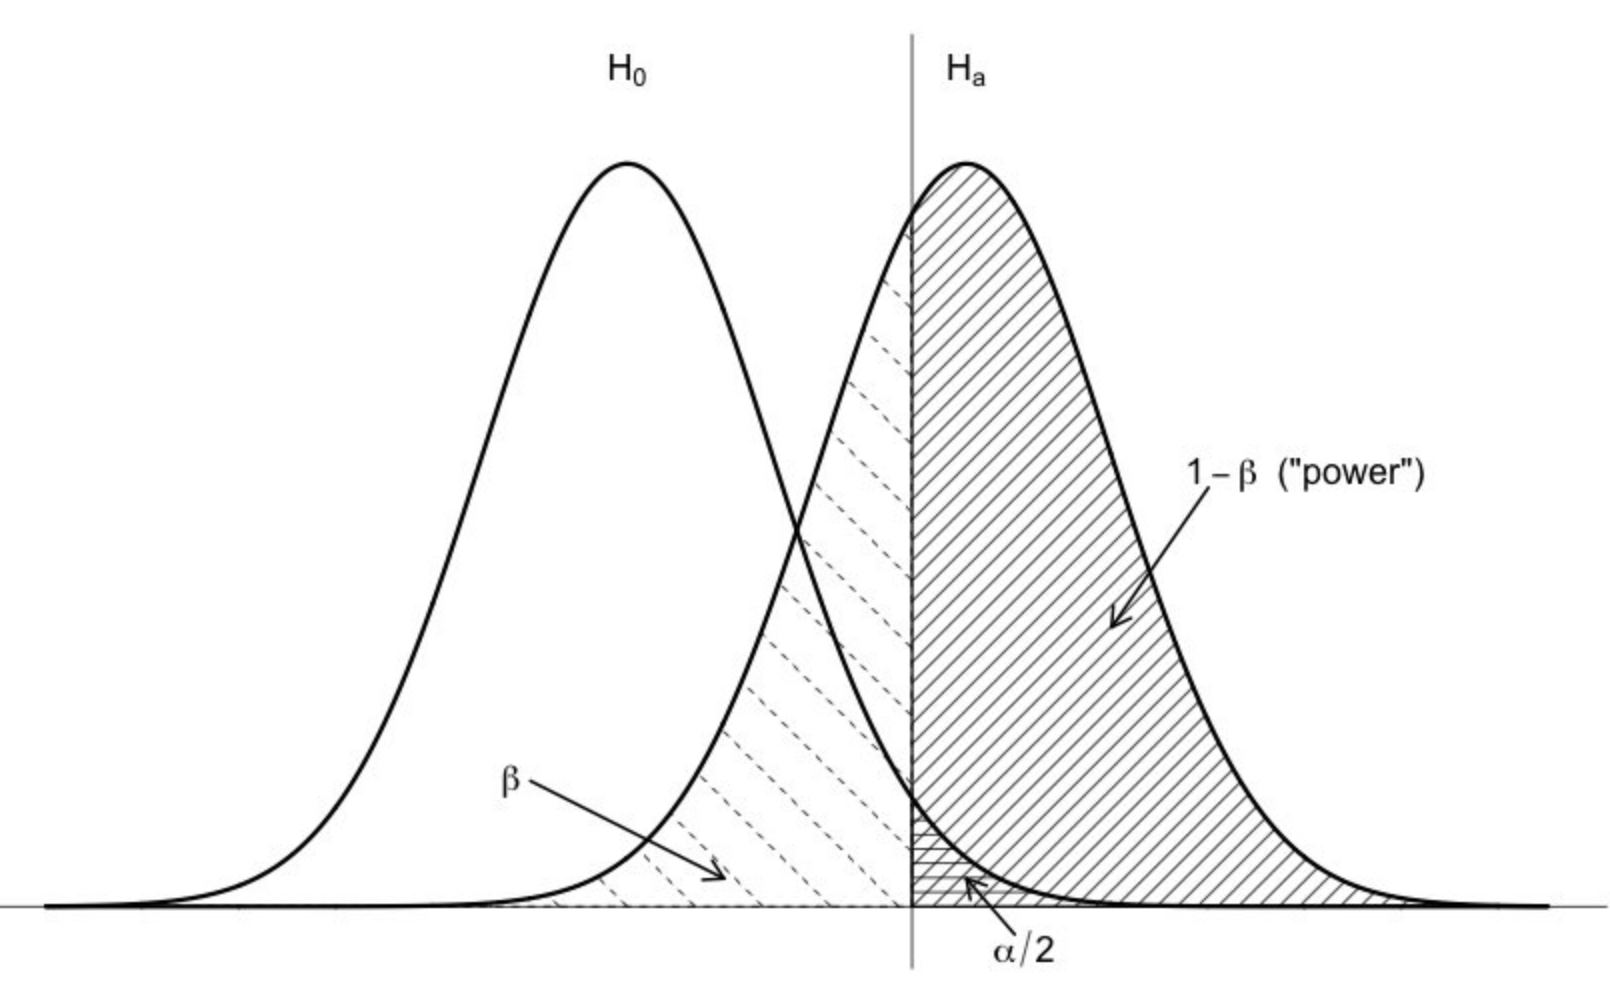
\includegraphics[width=\linewidth]{./figures/power}}
\end{center}
\end{frame}

\begin{frame}
  \frametitle{Statistical Power, Part II}
  
\end{frame} 

\begin{frame}
\frametitle{Statistical Power, Part III}

How to increase power
\begin{itemize}
\item Increase sample size.
\item Choose a powerful test (if you can justify its assumptions).
\end{itemize}

\end{frame}

\section{Practical Significance}

\begin{frame}
  \frametitle{Practical significance}
  \begin{block}{Statistical significance}
    \begin{itemize}
    \item How much does the data support the existence of an effect?
    \end{itemize}
  \end{block}
  \begin{block}{Practical significance}
    \begin{itemize}
    \item Is the size of this effect important?
    \item What is the magnitude of the effect?
    \item Should we care about this effect?
    \end{itemize}
  \end{block}
  \note[item]{In many cases, statistical significance is little more
    than a statement of how large a sample was used to test a
    question.}
\end{frame}
 
 \begin{frame}
   \frametitle{Example}
   \begin{exampleblock}{Productivity supplements}
     % Suppose that two studies examine how vitamin supplements affect
     % productivity.
     \vspace{1em}

     \begin{columns}[t]
       \column{0.42\textwidth}
       \textbf{Vitamin W}
       \begin{align*}
         n &= 30 \\ 
         \mu_{treat} &= 12.6 \\
         \mu_{control} & = 6.1 \\
         p &= 0.11
       \end{align*} 
        \textit{``The difference between groups was not
           statistically significant}, $(t=1.34, p=0.11$).''
       \column{0.42\textwidth}
       \textbf{Vitamin Q}
       \begin{align*}
         n &= 30,000 \\
         \mu_{treat} &= 6.25 \\
         \mu_{control} &= 6.21 \\
         p &= 0.0005
       \end{align*}
       \textit{``The difference between the two groups was highly
         significant}, $(t = 3.34, p<0.001)$.'' 
     \end{columns}
   \end{exampleblock}
 \end{frame}

 \begin{frame}
   \frametitle{Practical Significance: Context}
   \textbf{Primary goal}: Provide context for your audience to reason
   about results.
   \begin{itemize}
   \item Who is your audience? 
   \item What action might be taken based on these results?
   \item How does this result alter how you would run the business? 
   \item What is the cost-benefit for implementing a change based on
     this result? 
   \item How does this result ``stack up'' to other effects?
   \end{itemize}
   \note[item]{Understanding and communicating the business context is
     what separates good analysts from great data scientists.}
   \note[item]{One might be very certain of a very small increase in a
     desirable metric; one might be less certain of a very large
     increase in a desirable metric.} 
   \note[item]{In many places, every relationship examined is
     significant. But, what do they \textit{mean}?} 
   \note[item]{We should directly tie this in to the machine learning
     conversation they're going to have in 207 about feature
     importance.} 
 \end{frame}

 \begin{frame}
   \frametitle{Practical Significance: Model Explainability}
   \begin{itemize}
   \item Some tasks require \textit{explainable} models.
   \item Finance, healthcare, insurance, and other regulated industries
     stipulate specific model forms .
   \item Humans reason in linear hypotheses— higher-dimensional
     and conditional hypotheses are too much to keep in
     mind.
   \end{itemize}
 \end{frame}

\begin{frame}
  \frametitle{Practical Significance: Effect Sizes}
  \begin{block}{Effect sizes} 
    \begin{itemize}
    \item Single-number metrics that characterize the
      magnitude of an effect
    \item Population parameters that we estimate—\textit{do not vary
        based on sample size}
    \end{itemize}
  \end{block}
  \vspace{1em} 
  \begin{columns}[t]
    \column{0.49\linewidth}
    \textbf{Invalid effect size metrics}
    \begin{itemize}
    \item t-stat
    \item p-value 
    \end{itemize}
    \column{0.49\linewidth}
    \textbf{Valid effect size metrics} 
    \begin{itemize}
    \item Mean values 
    \item Difference in means between groups
    \end{itemize}
  \end{columns} 
% Headline Test: What single number can you put in a newspaper
% headline to get the importance across? 
% \begin{itemize}
% \item Ex: Vitamin W increases lifespan by 1.2 years.
% \end{itemize}
\note[item]{This headline test feels out of place relative to the
  other content on this section.}
\end{frame}

\begin{frame}
  \frametitle{Standard Effect Size Measures}
  Standardized effect sizes are designed to be flexible and apply in
  many scenarios:
  \begin{itemize}
  \item Cohen's $d$
  \item Correlation $\rho$
  \item Cramer's $V$
  \end{itemize}
  General metrics ignore the specific context around your research or
  business question.
  \note[item]{These provide general guidance about whether an effect
    is small, medium, or large.}  
  \end{frame}


\begin{frame}
  \frametitle{Cohen's d}
    Sometimes, a mean (or difference in means) is hard to assess because
  the units are unfamiliar.
  \begin{itemize}
  \item \textbf{Example}: The effect of angled bristles on tooth decay
    is 5 millicaviparsecs per
    brushstroke %% TO THE REVIEWERS: Yes, we know this isn't a word
  \end{itemize}
  \begin{block}{Cohen's d} 
    Compare effect size relative to the underlying natural variation
    in the outcome.
    \[
      \text{Cohen's } d = \frac{\text{mean difference}}{\text{standard
          deviation}}
    \]
    \end{block} 
\end{frame}

\begin{frame}
  \frametitle{Cohen's d (cont.)}
  \begin{center}
  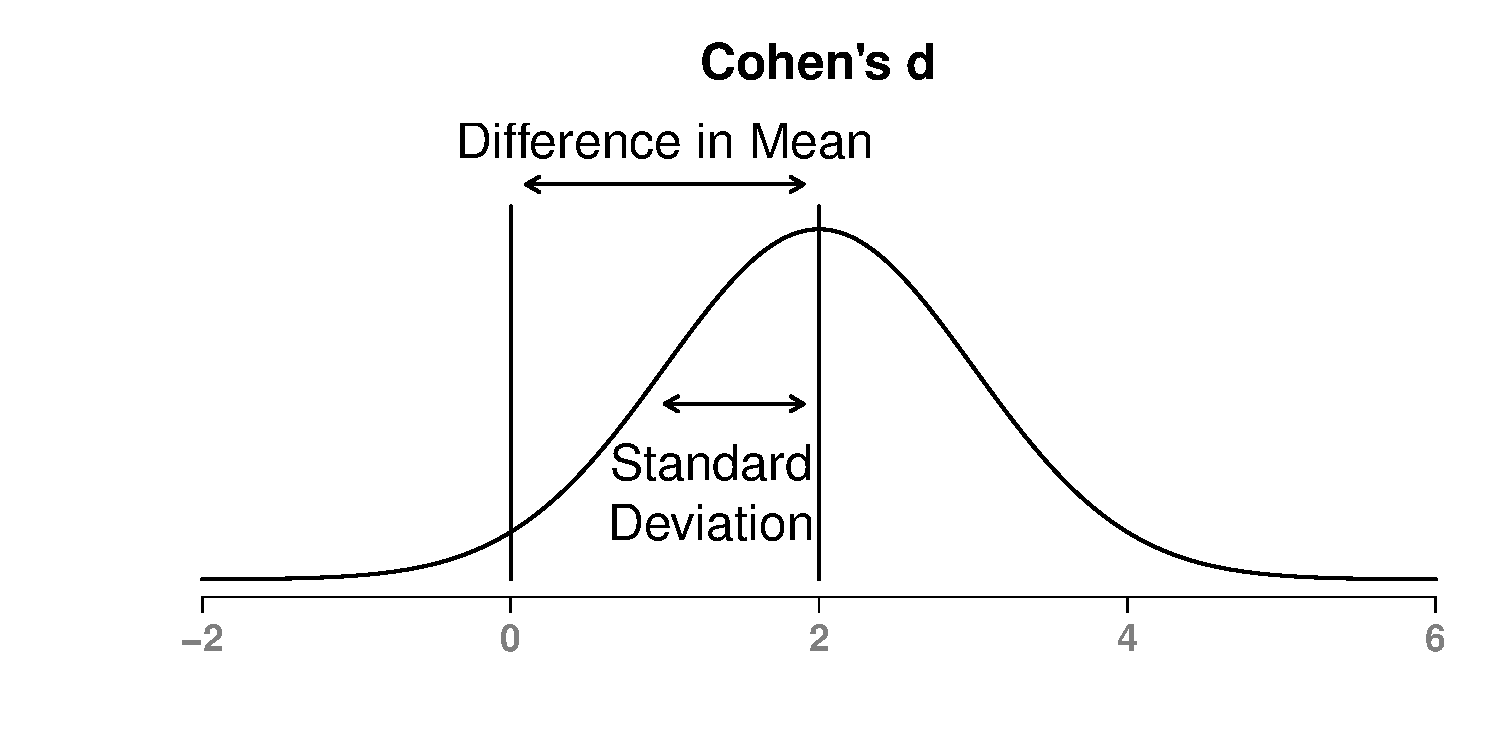
\includegraphics[width=\linewidth]{./figures/cohens_d.pdf}
  \end{center}
\end{frame} 

\begin{frame}
  \begin{block}{Rules of thumb (according to Cohen)}
    \begin{center}
      \begin{tabular}{rc}
        Small effect     & $d = 0.2$ \\ 
        Medium effect & $d = 0.5$ \\ 
        Large effect      & $d = 0.8$ \\
      \end{tabular}
    \end{center}
  \end{block} 
  \begin{itemize}
    \item Applicable across a huge number of contexts 
    \item Ignores any important differences between context 
    \item Saving dollars or saving lives are the same to Cohen's d
  \end{itemize} 
\end{frame}

\begin{frame}
  \frametitle{Takeaways}
  \begin{itemize}
  \item  After a statistical test, it's important to assess both
    statistical significance and practical significance.
  \item Standard effect size measures can help in a wide variety of situations.
  \item But don't get carried away and reach for them automatically.
  \item The main objective is to clearly explain how important the
    magnitude of the effect is.
  \end{itemize}
\end{frame}

\section{Guidelines for Statistical Reporting}

\begin{frame}
  \frametitle{Guidelines for Statistical Reporting}
  \begin{itemize}
    \item Communicating results is a \textit{key} part of statistical analysis.
    \item In this class, in other classes, and in your organization, you will be expected to submit your analysis as a written report.
  \end{itemize}
\end{frame}

\begin{frame}
  \frametitle{Guidelines}
  \begin{enumerate}
    \item A statistical analysis is a written argument.
    \item If you don't have something to say about some output, don't display it.
    \item Document every decision that you make.
    \item Identify features of the population that should be reflected in statistical models.
    \item Be clear about the difference between the sample and the population.
    \item The code is a part of the argument.
  \end{enumerate}
\end{frame}

\end{document}
